As it was stated in the introduction chapter of Section 1.1, the major research goal of this thesis is the construction of an automated solution for horizontal scalability problem which meets the SLA guarantees along with cost benefits. The approach taken to achieve this goal is presented in this chapter. This approach uses threshold based rules to scaling virtual machines horizontally by applying workload forecasting. To enable workload forecasting, ARIMA time series forecast strategy is applied periodically. The AppElastic autoscaling algorithm presented in this chapter works in collaboration with workload forecasting to proactively scale the system. This chapter revolves around the idea of ensuring SLA requirements by workload forecasting and scale the resource by threshold based rules.
\\
The proposed AppElastic algorithm is explained in three folds. First in Section~\ref{sub:AppElastic without look-ahead} an algorithm is developed as reactive provisioning solution to meet the SLA requirements for any workload. Next in Section~\ref{sub:AppElastic with look-ahead} algorithm is extended to provide a proactive scaling to solve the problem with VM provisioning latency. Finally, at the end of the Section~\ref{sub:AppElastic with look-ahead} complete AppElastic algorithm is presented.
\section{Assumptions and Limitations}
\label{sec:Assumptions and Limitations}
It is safe to assume that software monitoring services  such as Nagios~\cite{josephsen2007building} is able to monitor constantly and report the workload as user request arrive to the system. In this case time series forecast system can be applied to predict future workload points. Concerning the approach taken in this thesis, the input to time series based forecasting strategy assumes to be a time series of number of user requests arriving to the system. The time series forecasting mentioned in the following section is not meant to be applied on resource utilization, response time or any other throughput values.
\\
Going further in this thesis Amazon AWS is considered as a cloud service provider. As it was presented in table~\ref{table:cost}, Amazon AWS provides two types of instances, pay-per-use on-demand instances(ODI) and one-time/partial prepaid reserved instances(RI). These various instance purchasing option and cost model is used as an example in this thesis.
\\
Any time series forecasting strategy has an inheriting uncertainty due to unforeseeable system workload changes. It is obvious that system under drastic events can not be forecasted solely based on historical data \cite{herbst2012workload}. Influence of unplanned events can cause anomalies in the scaling decision that can be detected and analyzed afterwards.

\section{SLA Violations}
\label{sec:SLA Violations}
SLA aware provisioning is an important aspect for the service consumers and SLA violations are used to trigger scaling. Most of the works presented in related work chapter use SLA violations to trigger scaling either using proactive or reactive methods. SLA aware solutions are limited to providing some guarantees with respect to the service response time. In the scope of this thesis, SLA guidelines were given by industry partner Citrix Online Dresden. Based on extensive research conducted by Citrix Online team, SLA violations for its audio/video server were defined in terms of number users being served by audio/video servers. It was identified that, to meet SLA agreement for all its users, each server should server not more than 120 user in any given time. If server assigned more than 120 users, SLA agreement was being violated.

\section{AppElastic Algorithm}
\label{sec:AppElastic Algorithm}

\subsection{AppElastic without look-ahead}
\label{sub:AppElastic without look-ahead}

In this section AppElastic algorithm is introduced without the feature of workload forecasting. Algorithms strengths and weaknesses will also be discussed. In order to understand the algorithm better, Table~\ref{table:paratable} list the input parameters of the algorithm. First of all, the IaaS cloud providers has specific billing period for its instances. This value is specified with the parameter $B_{p}$. This billing period varies based on the cloud service providers. For example, Amazon AWS charges its customer instances in hourly basis\footnote{https://aws.amazon.com/ec2/pricing/}. In addition, users need to specify the time required to startup and shutdown a virtual machine as in $T_{startup}$ and $T_{shutdown}$ respectively. As explained in Chapter \ref{chap:Introduction}, each virtual machines has unpredictable long startup time\cite{mao2012performance}. This varied startup time are necessary to consider in AppElastic algorithm since it has a considerable delay in provisioning the VM for the application users to fulfill SLA requirements. VM shutdown time generally depends on the graceful shutdown of the application running inside VM and this value has to be specified based on experiments done based on specific application. In the scope of this thesis, industry partner Citrix online provided the VM instance startup time as 5 mins and, 15 mins for migrating its user  and completely shutdown the virtual machines.
\\
As it was defined, AppElastic algorithm is based on threshold based rules. AppElastic algorithm takes number of user session per VM instance as threshold specified by the parameter \( U_{i} \). This threshold is used for triggering scaling of VM. This threshold is determined by QoS demand requirements as per SLA. The pseudo code of the algorithm is given in \textit{Algorithm}~\ref{algo:appelasticwithoutlookahead}. Output values from  \textit{Algorithm}~\ref{algo:appelasticwithoutlookahead} are as shown in Table~\ref{table:outputtable}. It give two type of output, one is the usage of each VM instance through $VM_{usage}^{i}$ and cost associated with this usage in $VM_{cost}^{i}$. Algorithm is started after application is deployed and keeps running until application is completed. Scaleup is triggered when it observe the user requests growing above the specified threshold or scale down if the billing period of VM is ending and number of user session are below specified threshold.
\\
The algorithm applies an automatic reactive scaling mechanism similar to mechanisms applied by Amazon Auto Scale and Rightscale\cite{han2012lightweight}. The threshold based scaling need no prior knowledge about the application. Each time VM instances are scaled its load balancing server automatically redistributes incoming user request to new created instances\cite{han2012lightweight}. This algorithm tries to provide best service for all of its application users by creating as much VM instances needed. This algorithm is effected by the VM startup time, since there is an overhead in VM startup time, VM's cannot be made available by the scaling algorithm to the application users. As show in the Figure~\ref{fig:slaviolationfig}, due to a sudden increase in incoming user requests the scaling algorithm starts adding new machines, since VM has considerable startup time users were not served at this time and SLA is violated by not providing the service. This is evident from the Figure~\ref{figure:slavioa} and Figure~\ref{figure:slaviob}, number of VM's available to serve the user request are inadequate hence user request red dotted line does not fall under VM's capacity blue line. To solve this problem, we need a mechanism to predict user request for certain period, so that algorithm can look-ahead in time and add new VM instances which server all upcoming user requests without violating SLA.

\RestyleAlgo{boxruled}
\LinesNumbered
\begin{algorithm}[H]
 \KwIn{  \( U_{i} \),\( B_{p} \),\( T_{start} \),\( T_{shutdown} \)}
 \KwOut{$VM_{usage}^{i}$, $VM_{cost}^{i}$}
 \While{until application is active}{
  \tcc{user request \( r_{i} \) at time \(t_{i}\)}
  \(r_{i}  \) = getUserRequest()\;
  \tcc{machines \( n_{i} \) required at time \( t_{i} \)}
  \( n_{i} = r_{i} / U_{i} \)\;
  \tcc{machines already running \( m_{i} \) at time \( t_{i} \)}
  \( m_{i} = getRunningVmInstanceCount() \)\;
  \uIf{\( n_{i} > m_{i} \)}{
    \tcc{Add more machines}
    \(newMachinesToStart =  n_{i} - m_{i}\)\;
    \lFor{ i=1 \emph{\KwTo} newMachinesToStart }{
    \tcc{New VM takes \( T_{start}\) mins to start}
    start new VM instance
    }
   }
   \uElseIf{\( n_{i} < m_{i} \)}{
    \(machinesToShutdown =  m_{i} - n_{i}\)\;
    \tcc{Stop machine before billing period to avoid billing to next hour and machines take \( T_{shutdown}\) mins to shutdown. Only stop machines which are nearning billing period.}
    \lFor{ i=1 \emph{\KwTo} machinesToShutdown }{ Stop VM instance ending billing period }
  }
 }
 \caption{AppElastic Algorithm without look-ahead}
 \label{algo:appelasticwithoutlookahead}
\end{algorithm}

\begin{center}
  \begin{table}
    \begin{tabular}{ | L{6cm} | L{6cm} |}
      \hline
      Parameter & Description \\ \hline
      \( U_{i} \) & Number of user session a single instance can accommodate  \\ \hline
      \( B_{p} \) & Billing period of instance as per cloud service provider policy \\ \hline
      \( T_{start} \) & Time taken for a VM and its application to start  and update its states if necessary  \\ \hline
      \( T_{shutdown} \) & Time taken for VM instance shutdown\\ \hline
    \end{tabular}
    \caption{List of input parameters to \textit{Algorithm}~\ref{algo:appelasticwithoutlookahead}}
     \label{table:paratable}
\end{table}
\end{center}

\begin{center}
  \begin{table}
    \begin{tabular}{ | L{6cm} | L{6cm} |}
      \hline
      Parameter & Description \\ \hline
      $VM_{usage}^{i}$ & Usage of each $VM_{i}$ in minutes  \\ \hline
      $VM_{cost}^{i}$ & Cost of $VM_{i}$ for its usage \\ \hline
    \end{tabular}
    \caption{List of out values from \textit{Algorithm}~\ref{algo:appelasticwithoutlookahead} and \textit{Algorithm}~\ref{algo:appelasticwithlookahead}}
     \label{table:outputtable}
\end{table}
\end{center}


\subsection{AppElastic with look-ahead}
\label{sub:AppElastic with look-ahead}
\subsubsection{Workload Forecasting Technique}
\label{subs:Workload Forecasting Technique}
To illustrate the process of time series modeling, workload from audio/video conferencing server logs is analyzed. To analyze the workload using time series model, the user requests are captured in the form of discrete time series values. Actual workload to the algorithm is be depicted in the Figure~\ref{figure:sampleworkload}. As discussed earlier, each point represents the total number of requests for each minute. The workload is captured every minute, hence the scaling decision would be taken at the interval of one minute and thus the forecast has to be done for next minutes. For  modeling of time series and forecasting workload, ARIMA model which was introduced in section~\ref{sub:ARIMA}.
To find the order of the model, that is to identify the values for $p$, $d$ and $q$, \(R\) statically software is used. The forecast package for \(R\) software developed by Hyndman et al.\cite{hyndman2007automatic} uses AIC, AICc or BIC values\cite{hyndman2007automatic} for $p$, $d$ and $q$ in ARIMA . The function \(auto.arima()\) searches the optimal number for ARIMA order. Using this software package the process of modeling and forecasting can be easily automated.
\\
To forecast the workload, the model developed above is used for prediction with some confidence interval. In this thesis, the model build as a automated process and can be best described through an algorithm. Forecasting algorithm is as show in the \textit{Algorithm}~\ref{algo:forecastalgo}. The parameters to this algorithm can be described in the Table~\ref{table:forecastparameter}. In the scope of this thesis, the algorithm is initialized with time series of 2500 points and the modeling is repeated every 5 mins or 15 mins based on the values specified by the forecast interval \(i\). Every forecast interval, new values from actual workload is included to the series to build a new model. This process of forecast will take place until the application is active. As mentioned above R forecast package is used to develop a best model. The forecasted data is written to a file so that the autoscaling algorithm can read the forecasted data. The Figure~\ref{figure:forecasted}  shows the forecast based on the model constructed above. In this study, 2500 observation are used to construct the model and it is used for forecasting and testing for next 2500 observations. While forecasting next 2500 observations,  interval of 5 minutes is used and new values of actual workload are included for successive models. Dotted red lines show the observed values and blue dotted line are the forecasted values with 0\% confidence interval. The evaluation of the model will be discussed in detailed in later chapters. This forecasting model will enable the AppElastic algorithm to look-ahead in time for making scaling decisions and avoid SLA violations.

\begin{flushleft}
  \begin{table}
    \begin{tabular}{ | L{5cm} | L{5cm} |}
      \hline
      Parameter & Description \\ \hline
      Time series & Number of user request as time series data \\ \hline
      Forecast Interval & A positive integer \(i\). Every \(i\) minutes new time series points in the time series arrivals and a forecast will be triggered. \\ \hline
      Forecast Horizon & Positive integer values quantifying the number of time series points to forecast.  \\ \hline
      Confidence Level(optional)  & An interval \([0,100)\) for forecast confidence.\\ \hline
    \end{tabular}
    \caption{List of input parameters to \textit{Algorithm}~\ref{algo:forecastalgo}}
     \label{table:forecastparameter}
\end{table}
\end{flushleft}

\RestyleAlgo{boxruled}
\LinesNumbered
\begin{algorithm}[H]
 \KwIn{time series \(t_i\), forecast interval \(i\), forecast horizon \(horizon\) }
 \KwOut{Predicted workload for forecast horizon \(horizon\) every forecast interval \(i\)}
 initialize \(R\) software, \(forecast\) library \;
 \While{until application is active and every \(i\) intervals}{
  \tcc{user request time series \( t_{i} \)}
  \tcc{using \(R\) software and package \(forecast\)}
  \( t_{i} \) = get new user request \;
  model = \(auto.arima(t_{i})\)\;
  forecastdata = \(forecast(t_{i}), h=horizon\)\;
  write forecast data to file \;

 }
  \caption{Workload forecasting algorithm}
  \label{algo:forecastalgo}
 \end{algorithm}

\subsubsection{AppElastic with Look-ahead}
\label{subs:AppElastic with Look-ahead}
As discussion in the previous section, VM startup time effects the SLA due to the fact that VM newly created takes time to start and  it is not immediately available for the application users. To mitigated this effect, a look in to the future workload could help in provisioning the VM before hand. The forecasting of user request workload discussed before will be used to forecast future workloads so that AppElastic algorithm has capability to look ahead and scale the VM instances. \textit{Algorithm}~\ref{algo:appelasticwithoutlookahead} presented in previous section is extended to have lookahead feature. This extended algorithm is as shown in  \textit{Algorithm}~\ref{algo:appelasticwithlookahead}. Compared to  \textit{Algorithm}~\ref{algo:appelasticwithoutlookahead}, \textit{Algorithm}~\ref{algo:appelasticwithlookahead} takes two additional parameter as described in Table~\ref{table:algo2paratable}. The parameter \( Lookahead_{scaleup} \) is an integer value used for lookahead in future workload for scaling  up. The threshold for scale up is modified according to this value. The scaleup threshold is calculated based on the maximum users in the forecast interval \( Lookahead_{scaleup} \). This is done to include all the user in the forecast interval and to make sure there are no SLA violations. Parameter \( Lookahead_{scaledown} \) is also an integer value used for lookahead in future workload while scaling down. These values are adjusted based on the VM startup and shutdown times. Even though users of this algorithm are free to choose any value, it is recommended in this thesis to use VM startup time for \( Lookahead_{scaleup} \) and VM shutdown+startup time for \( Lookahead_{scaledown} \). When VM startup time is used for scaleup, the autoscaling algorithm will lookahead for that duration and make the VM available for upcoming workload. Furthermore, scale down lookahead will helps in avoiding rapid VM starting and stopping by AppElastic algorithm. VM's which are already running will be extended to next billing cycle and reuse the already started VM instances.


\begin{flushleft}
  \begin{table}
    \scalebox{1}{
    \begin{tabular}{ | L{5cm} | L{5cm} | L{5cm} |}
      \hline
      Parameter & Description \\ \hline
      \( Lookahead_{scaleup} \) & Time interval for lookahead for scaling up \\ \hline
      \( Lookahead_{scaledown} \) & Time interval for lookahead for scaling down\\ \hline
    \end{tabular}
    }
    \caption{Additional input parameters to \textit{Algorithm}~\ref{algo:appelasticwithlookahead}}
     \label{table:algo2paratable}
\end{table}
\end{flushleft}

\subsubsection{AppElastic}
\label{subs:AppElastic}
Until now, AppElastic algorithm was discussed based on the scalability perspective. But one of the main goals of this thesis remain to be solved. The problem of choosing right instance type for a particular use case is till needed to be addressed.  IaaS cloud provider offers diverse instance purchasing options. As discussed in Chapter 1, a user can either run instances on demand and pay only for what is used or he can prepay to reserved instances for long so that he can avail some discount. There  exist few strategies as discussed in literature\cite{wang2013reserve}, but there is no silver bullet for solving this problem. However in the scope of this thesis, historical workload traces are useful to observe production application and VM instance usage. Based on heuristic technique, number of reserve instance used is varied, to find the optimal combination of reserver instance and on-demand instances by running AppElastic on the historical workload. Based on this heuristic technique, an optimal number is proposed to the user of the algorithm for choosing right number of reserving instances based on the cost benefits. Based on this requirement AppElastic with forecasting is extended to include two instance types and its purchasing cost. The complete AppElastic algorithm is as show in \textit{Algorithm}~\ref{algo:appelastic}. The new algorithm considers two instance types: Reserved instances (RI) and On-demand instances (ODI) and hence its instances are grouped into two separate lists. The cost associated with these two instances are passed as parameter via $Cost_{ri}$ and $Cost_{odi}$ for RI and ODI instances respectively. AppElastic user specifies the number of reserved instances to use so that it can calculate the cost incurred or saved by reserving an instance. Along with the number of reserved instances to use, the AppElastic also required the prices for each instance type in terms of effective hourly billing cost specified in US dollars as specified in Table~\ref{table:cost}. The input parameter to \textit{Algorithm}~\ref{algo:appelastic} are as shown in Table~\ref{table:appelasticparatable}. \textit{Algorithm}~\ref{algo:appelastic} need additional three parameters when compared to \textit{Algorithm}~\ref{algo:appelasticwithlookahead}. $Cost_{ri}$ and $Cost_{odi}$ are the cost of RI and ODI instances respectively. $Count_{ri}$ is the total RI instances to use. Value of $Count_{ri}$ is identified through heuristics approach described before and this process is automated in ElasticSim simulator. The idea behind the scaling remains the same from \textit{Algorithm}~\ref{algo:appelasticwithlookahead}. On successful completion, total cost of reserved instances and total cost of on-demand instances are provided as output. These output values are as described in Table~\ref{table:outputtableodiri}.

\begin{center}
  \begin{table}
    \begin{tabular}{ | L{6cm} | L{6cm} |}
      \hline
      Parameter & Description \\ \hline
      \( U_{i} \) & Number of user session a single instance can accommodate  \\ \hline
      \( B_{p} \) & Billing period of instance as per cloud service provider policy \\ \hline
      \( T_{start} \) & Time taken for a VM and its application to start  and update its states if necessary  \\ \hline
      \( T_{shutdown} \) & Time taken for VM instance shutdown\\ \hline
      $Lookahead_{scaleup}$ & Time interval to lookahead for scaling up \\ \hline
      $Lookahead_{scaledown}$ & Time interval to lookahead for scaling down \\ \hline
      $Cost_{ri}$ & Cost of RI instances as per Amazon AWS pricing as per Table~\ref{table:cost} \\ \hline
      $Cost_{odi}$ & Cost of ODI instances as per Amazon AWS pricing as per Table~\ref{table:cost} \\ \hline
      $Count_{ri}$ & Total number of RI instances to use \\ \hline
    \end{tabular}
    \caption{List of input parameters to \textit{Algorithm}~\ref{algo:appelastic}}
     \label{table:appelasticparatable}
\end{table}
\end{center}

\begin{center}
  \begin{table}
    \begin{tabular}{ | L{6cm} | L{6cm} |}
      \hline
      Parameter & Description \\ \hline
      $VM_{usage}^{i}$ & Usage of each $VM_{i}$ in minutes  \\ \hline
      $VM_{cost}^{i}$ & Cost of $VM_{i}$ for its usage \\ \hline
      $Total_{cost}^{ri}$ & Total cost of RI instances \\ \hline
      $Total_{cost}^{odi}$ & Total cost of ODI instances \\ \hline
    \end{tabular}
    \caption{List of out values from \textit{Algorithm}~\ref{algo:appelastic}}
     \label{table:outputtableodiri}
\end{table}
\end{center}

\begin{figure}
     \centering
     \begin{subfigure}[b]{0.7\textwidth}
         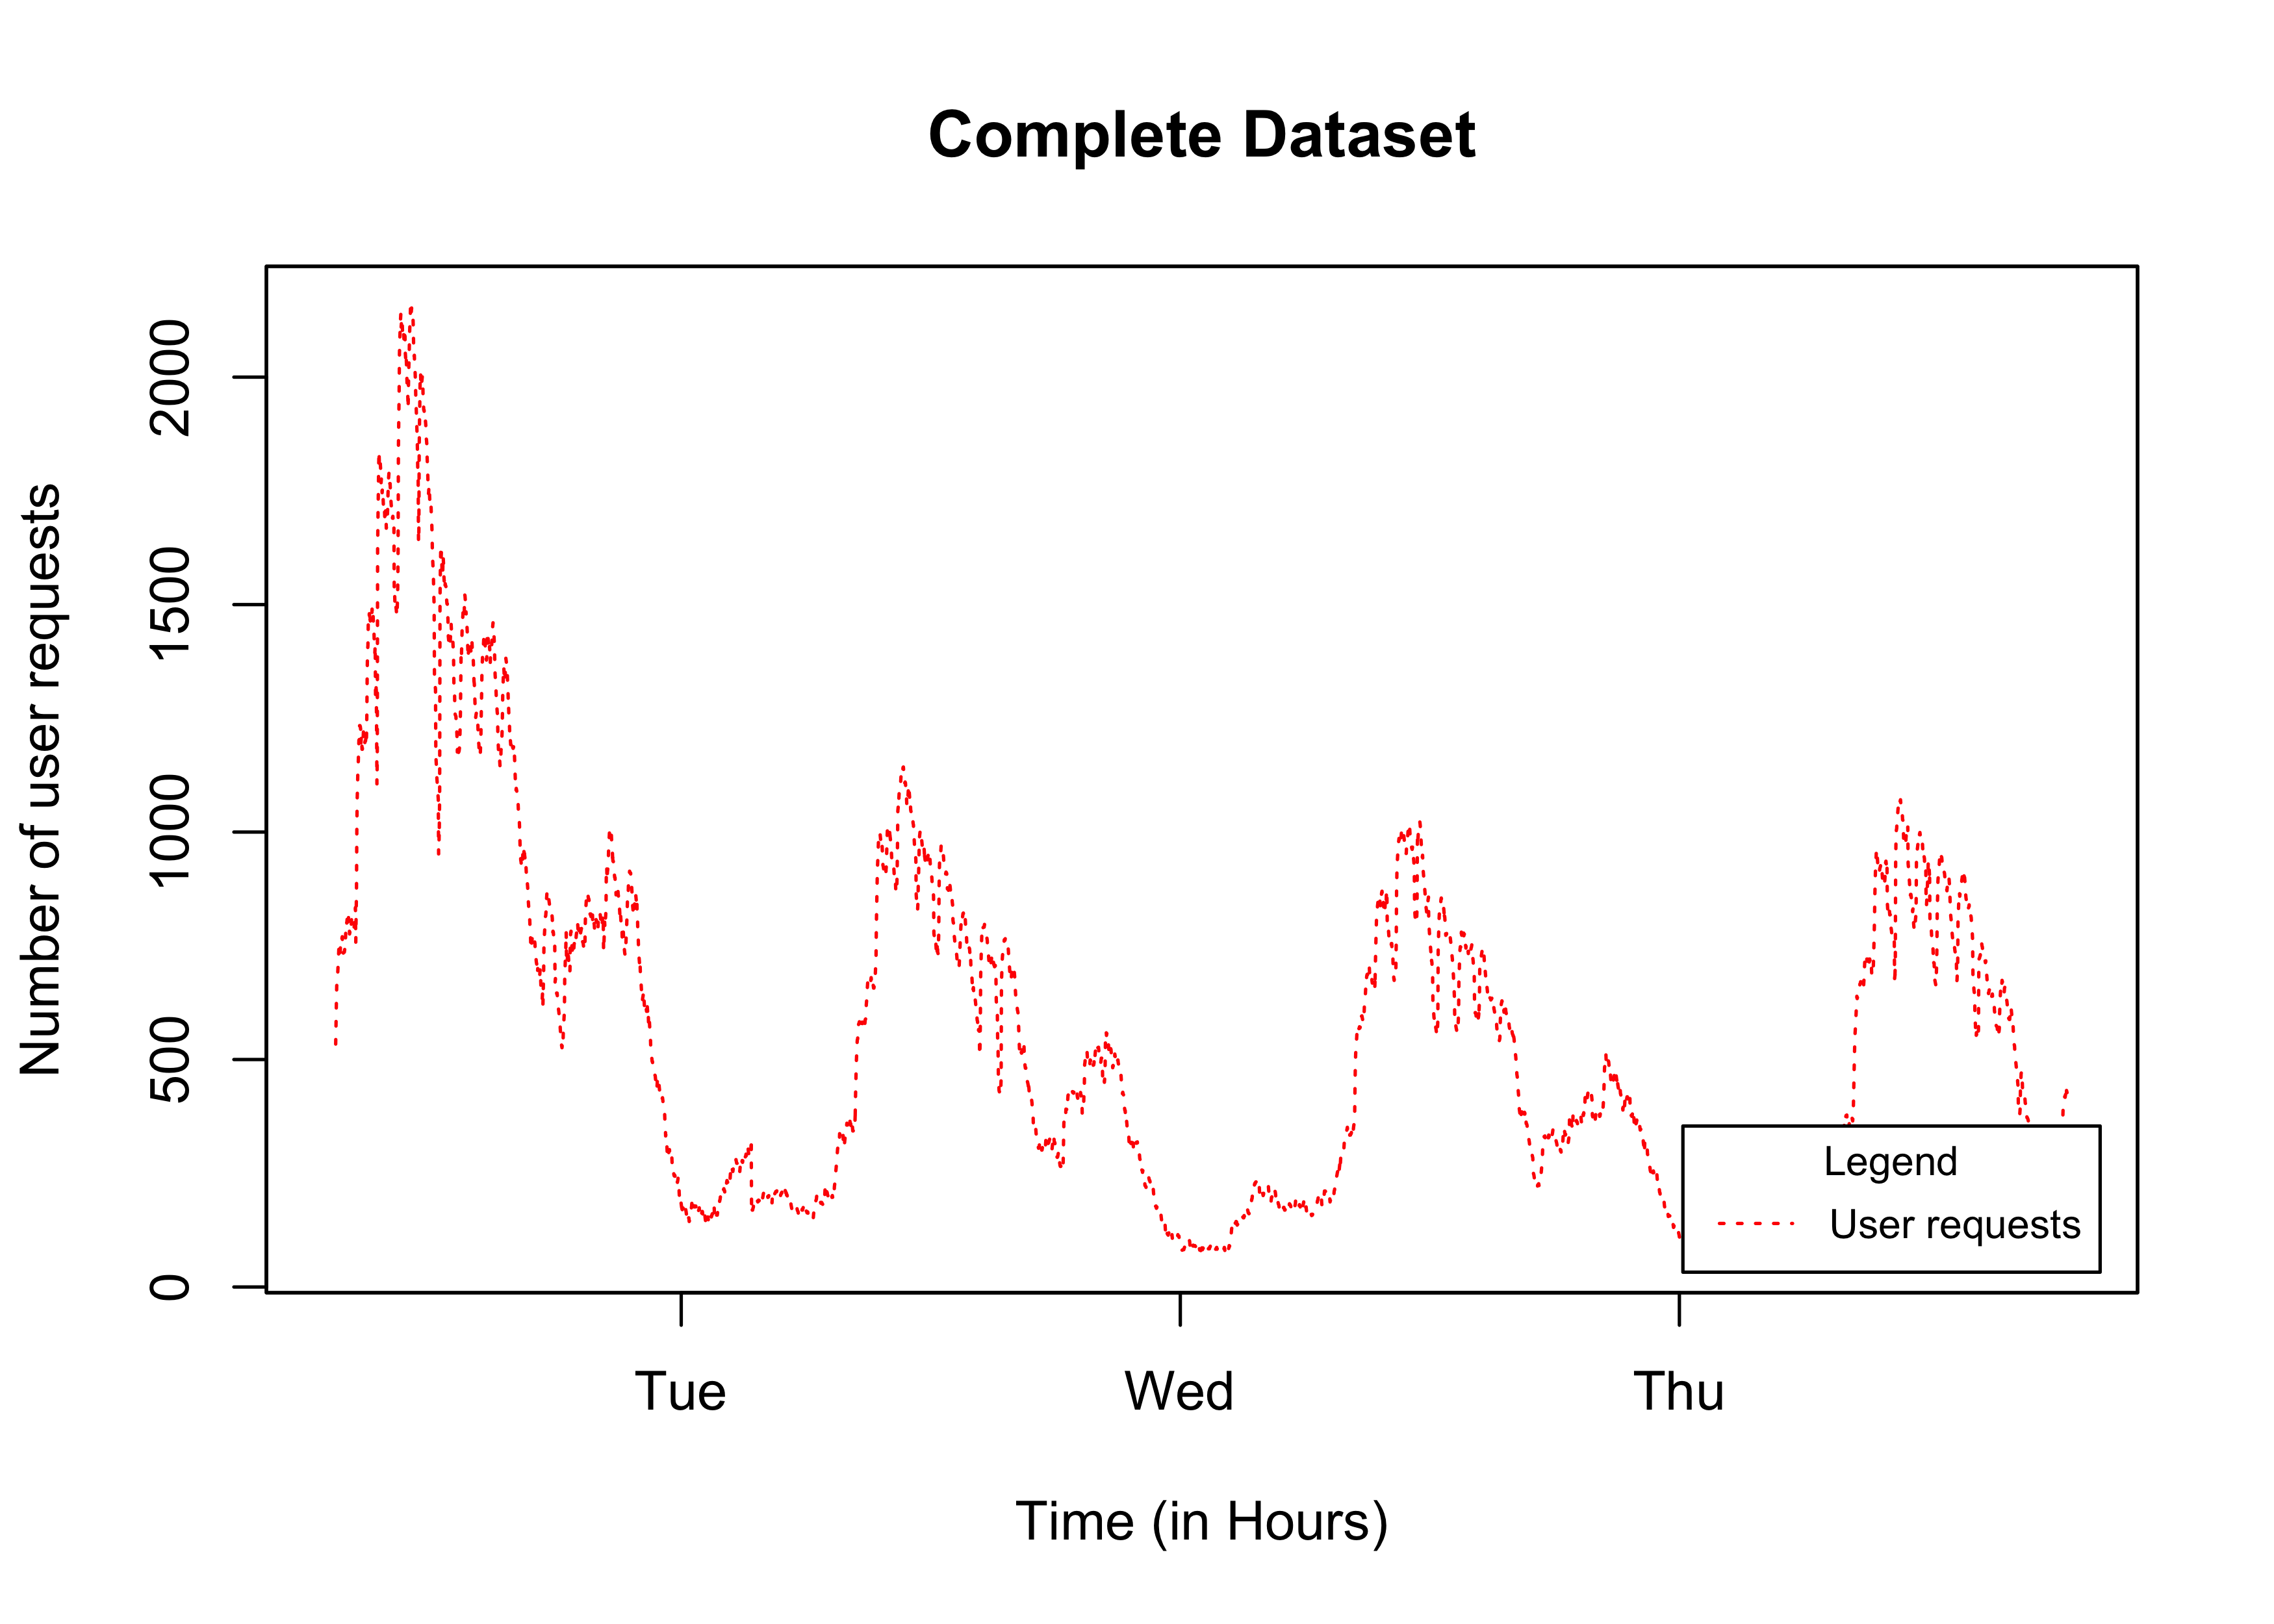
\includegraphics[width=\textwidth]{CompleteWorkload.png}
         \caption{Complete dataset}
         \label{figure:sampleworkload}
     \end{subfigure}
     \begin{subfigure}[b]{0.7\textwidth}
         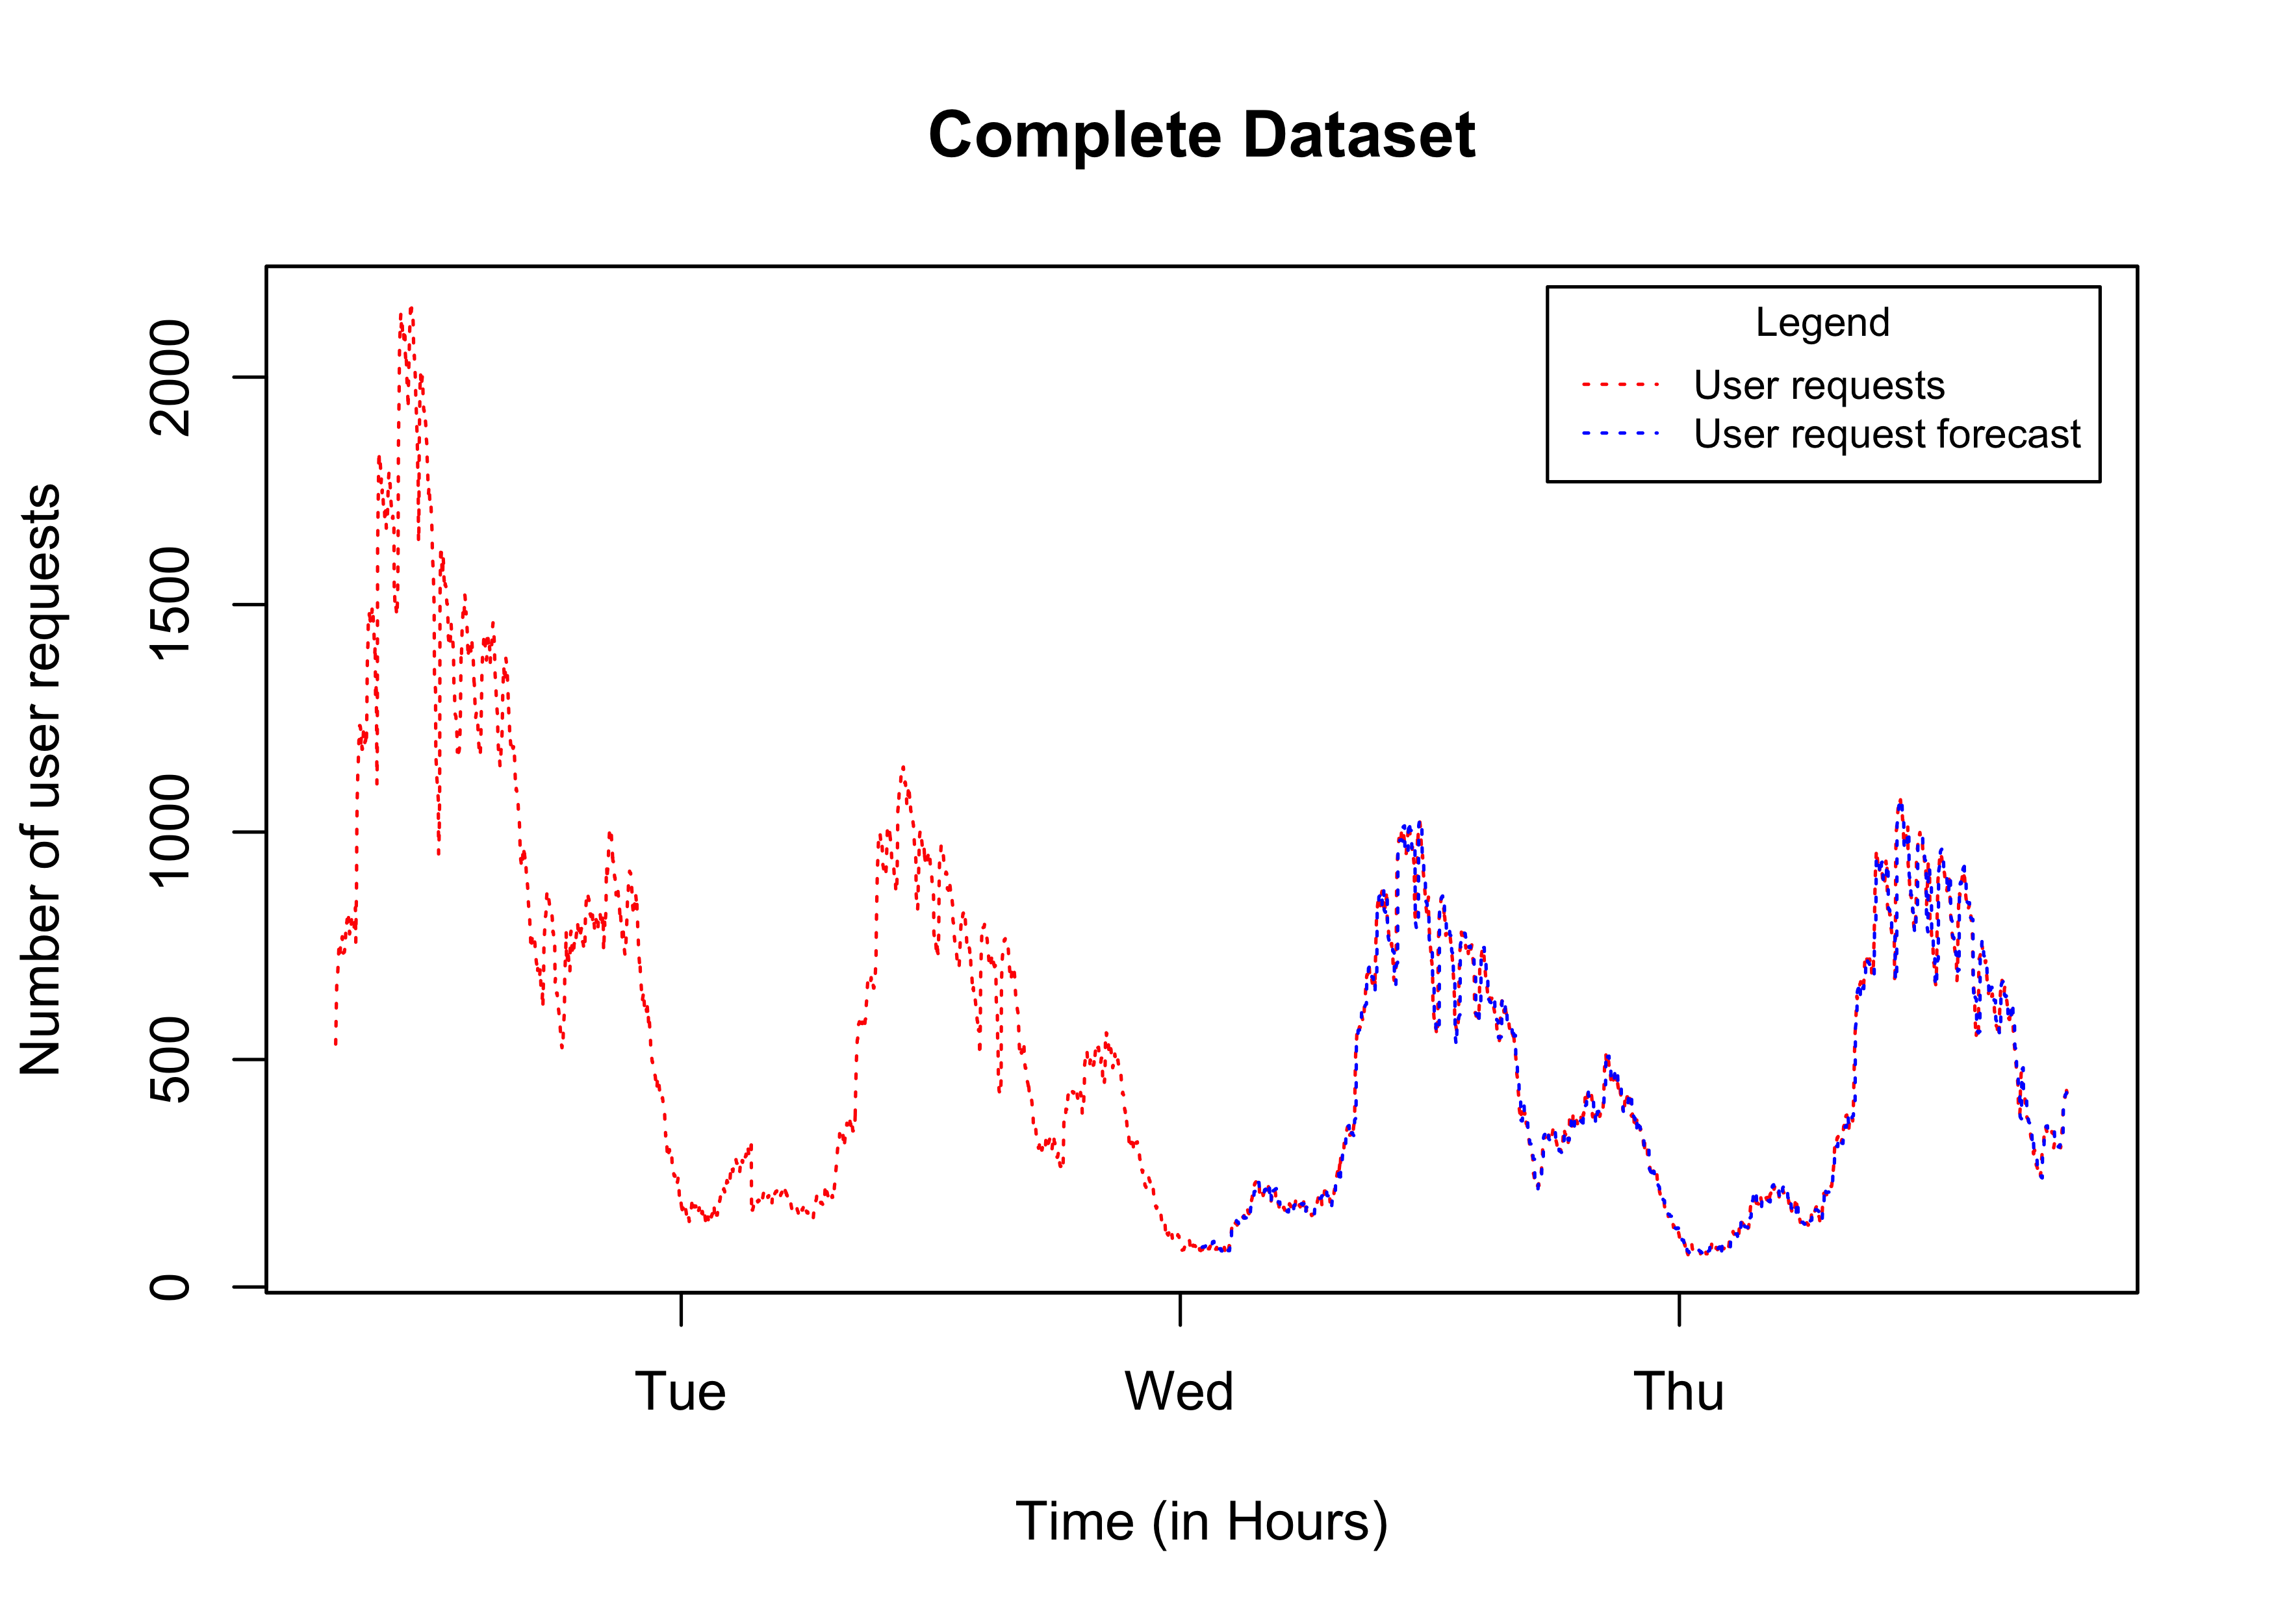
\includegraphics[width=\textwidth]{CompleteWithForecast.png}
         \caption{Actual and forecast dateset}
         \label{figure:forecasted}
     \end{subfigure}
     \caption{Workload observed and forecasted}
     \label{fig:workloads}
 \end{figure}
 \begin{figure}
      \centering
     \begin{subfigure}[b]{0.6\textwidth}
         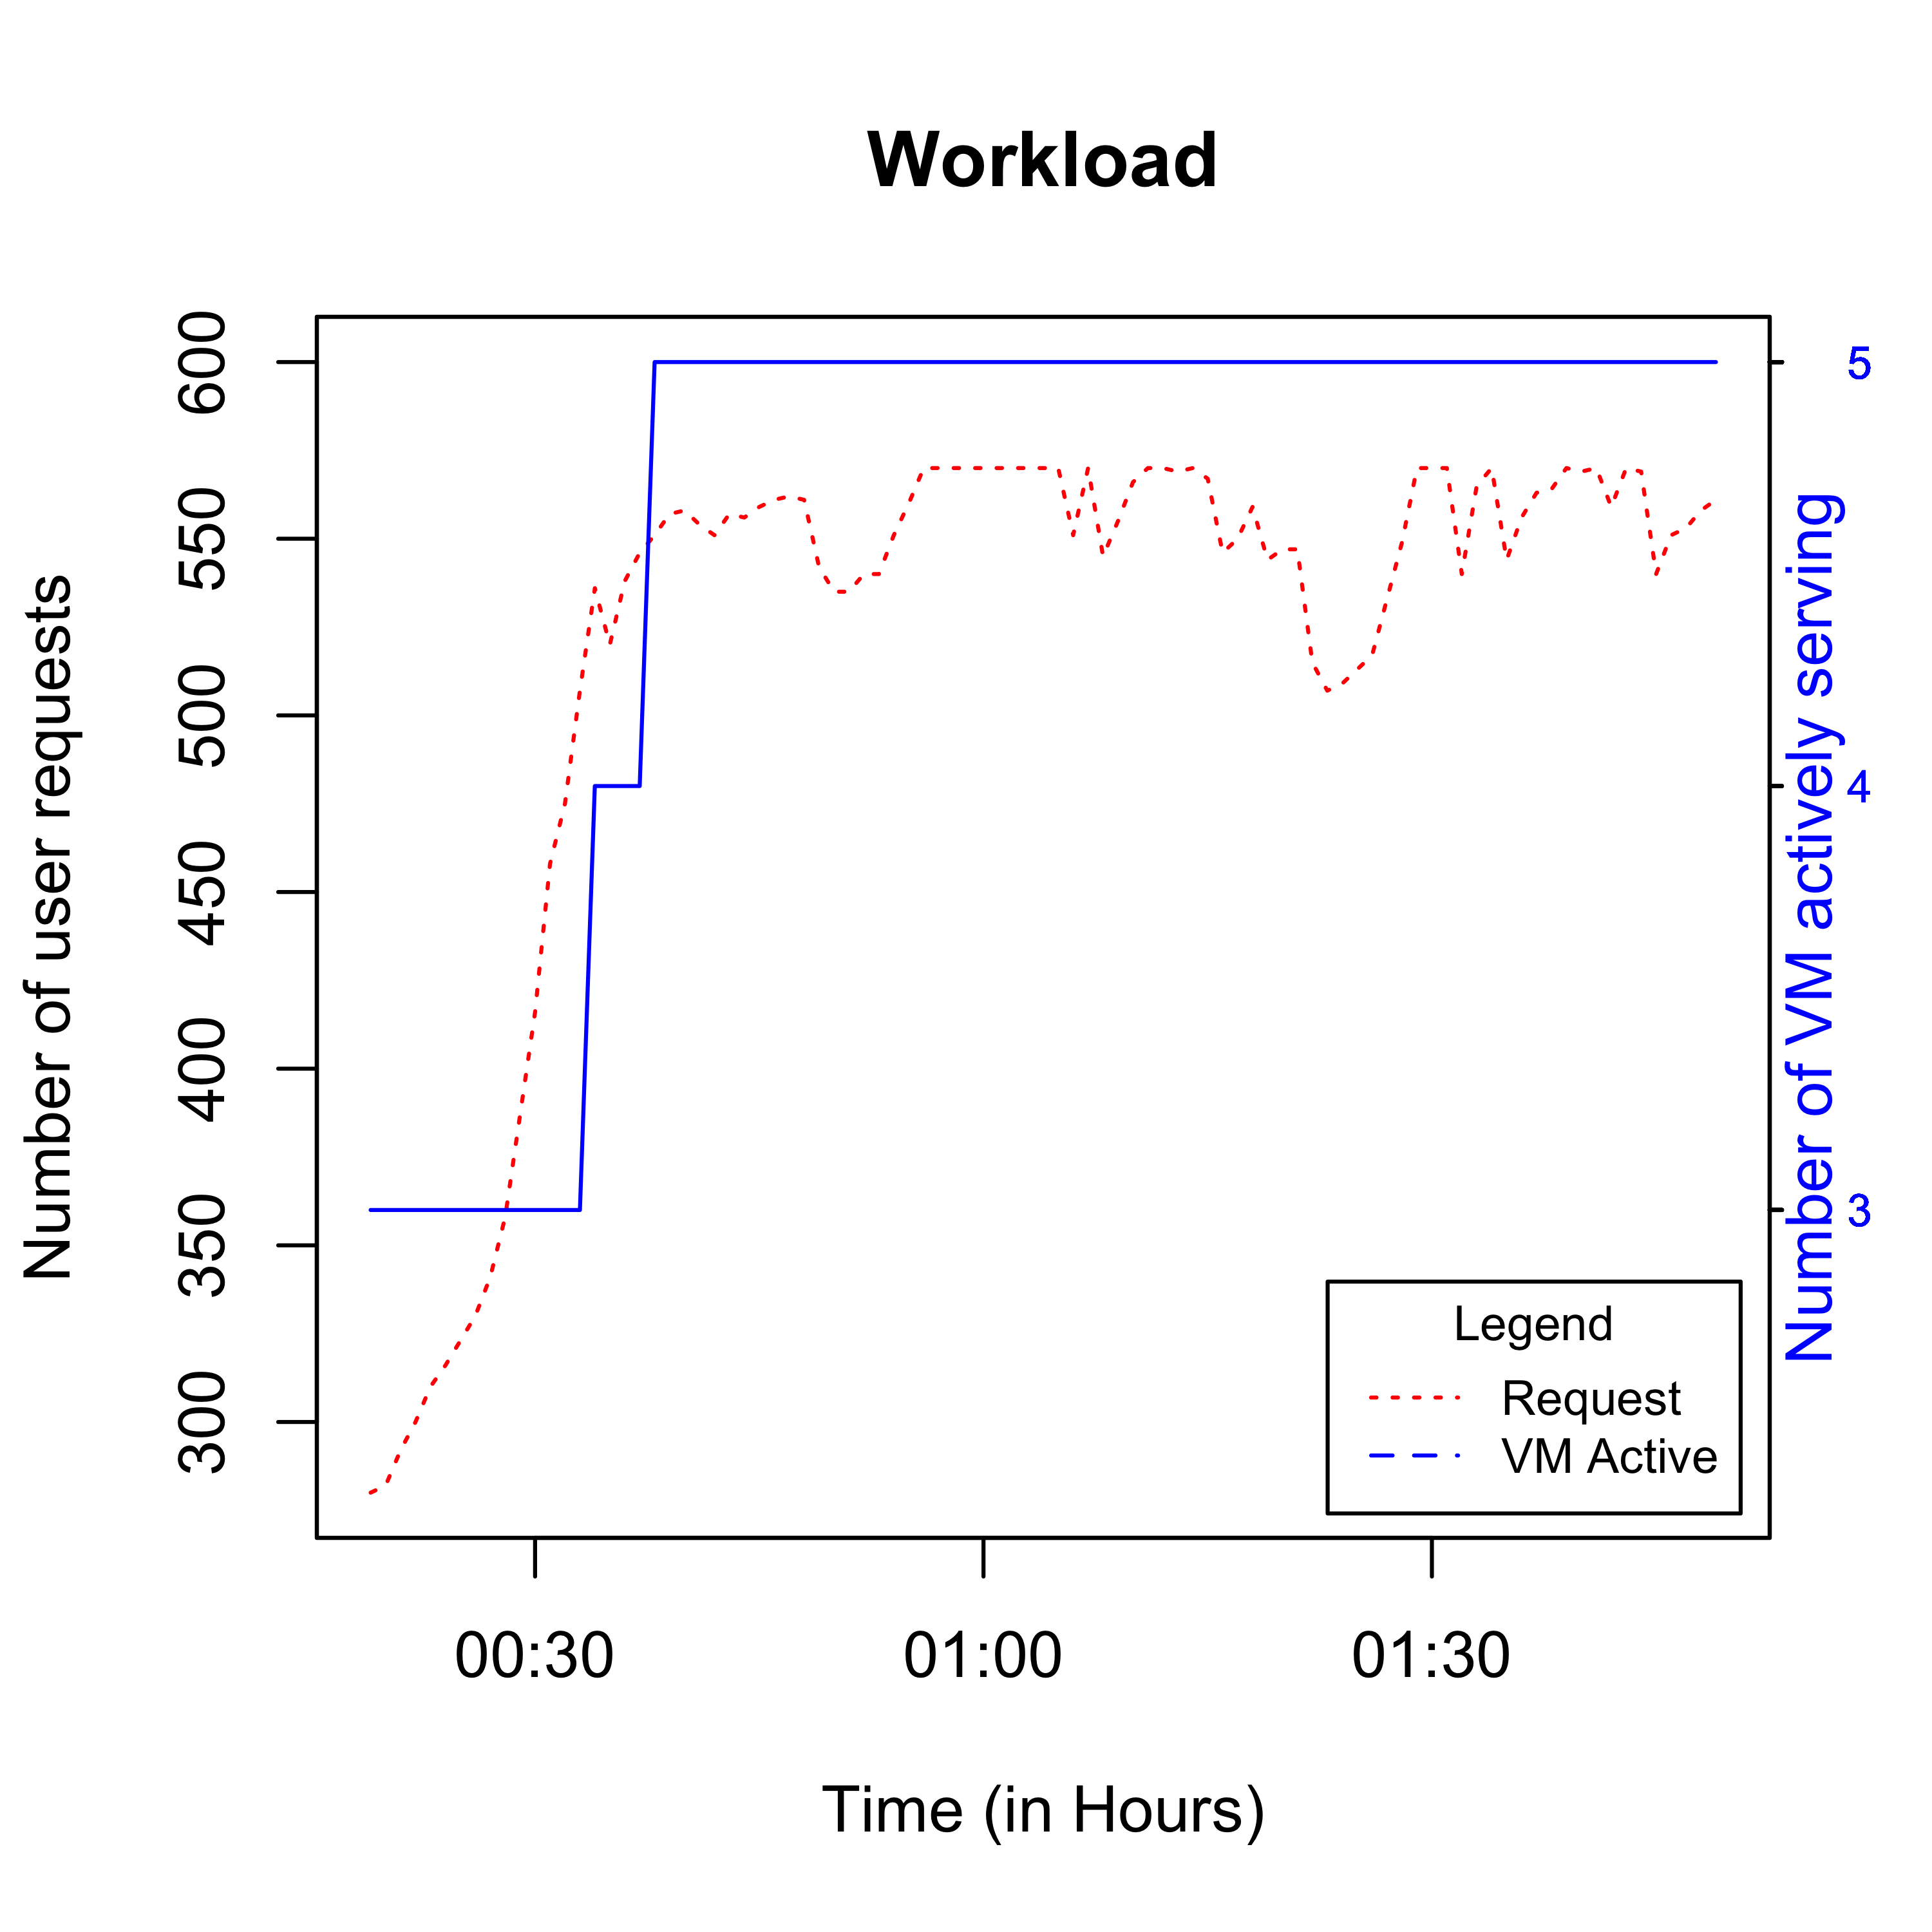
\includegraphics[width=\textwidth]{slaviolationfront.png}
         \caption{SLA Violation exmaple-1}
         \label{figure:slavioa}
     \end{subfigure}
     \begin{subfigure}[b]{0.6\textwidth}
         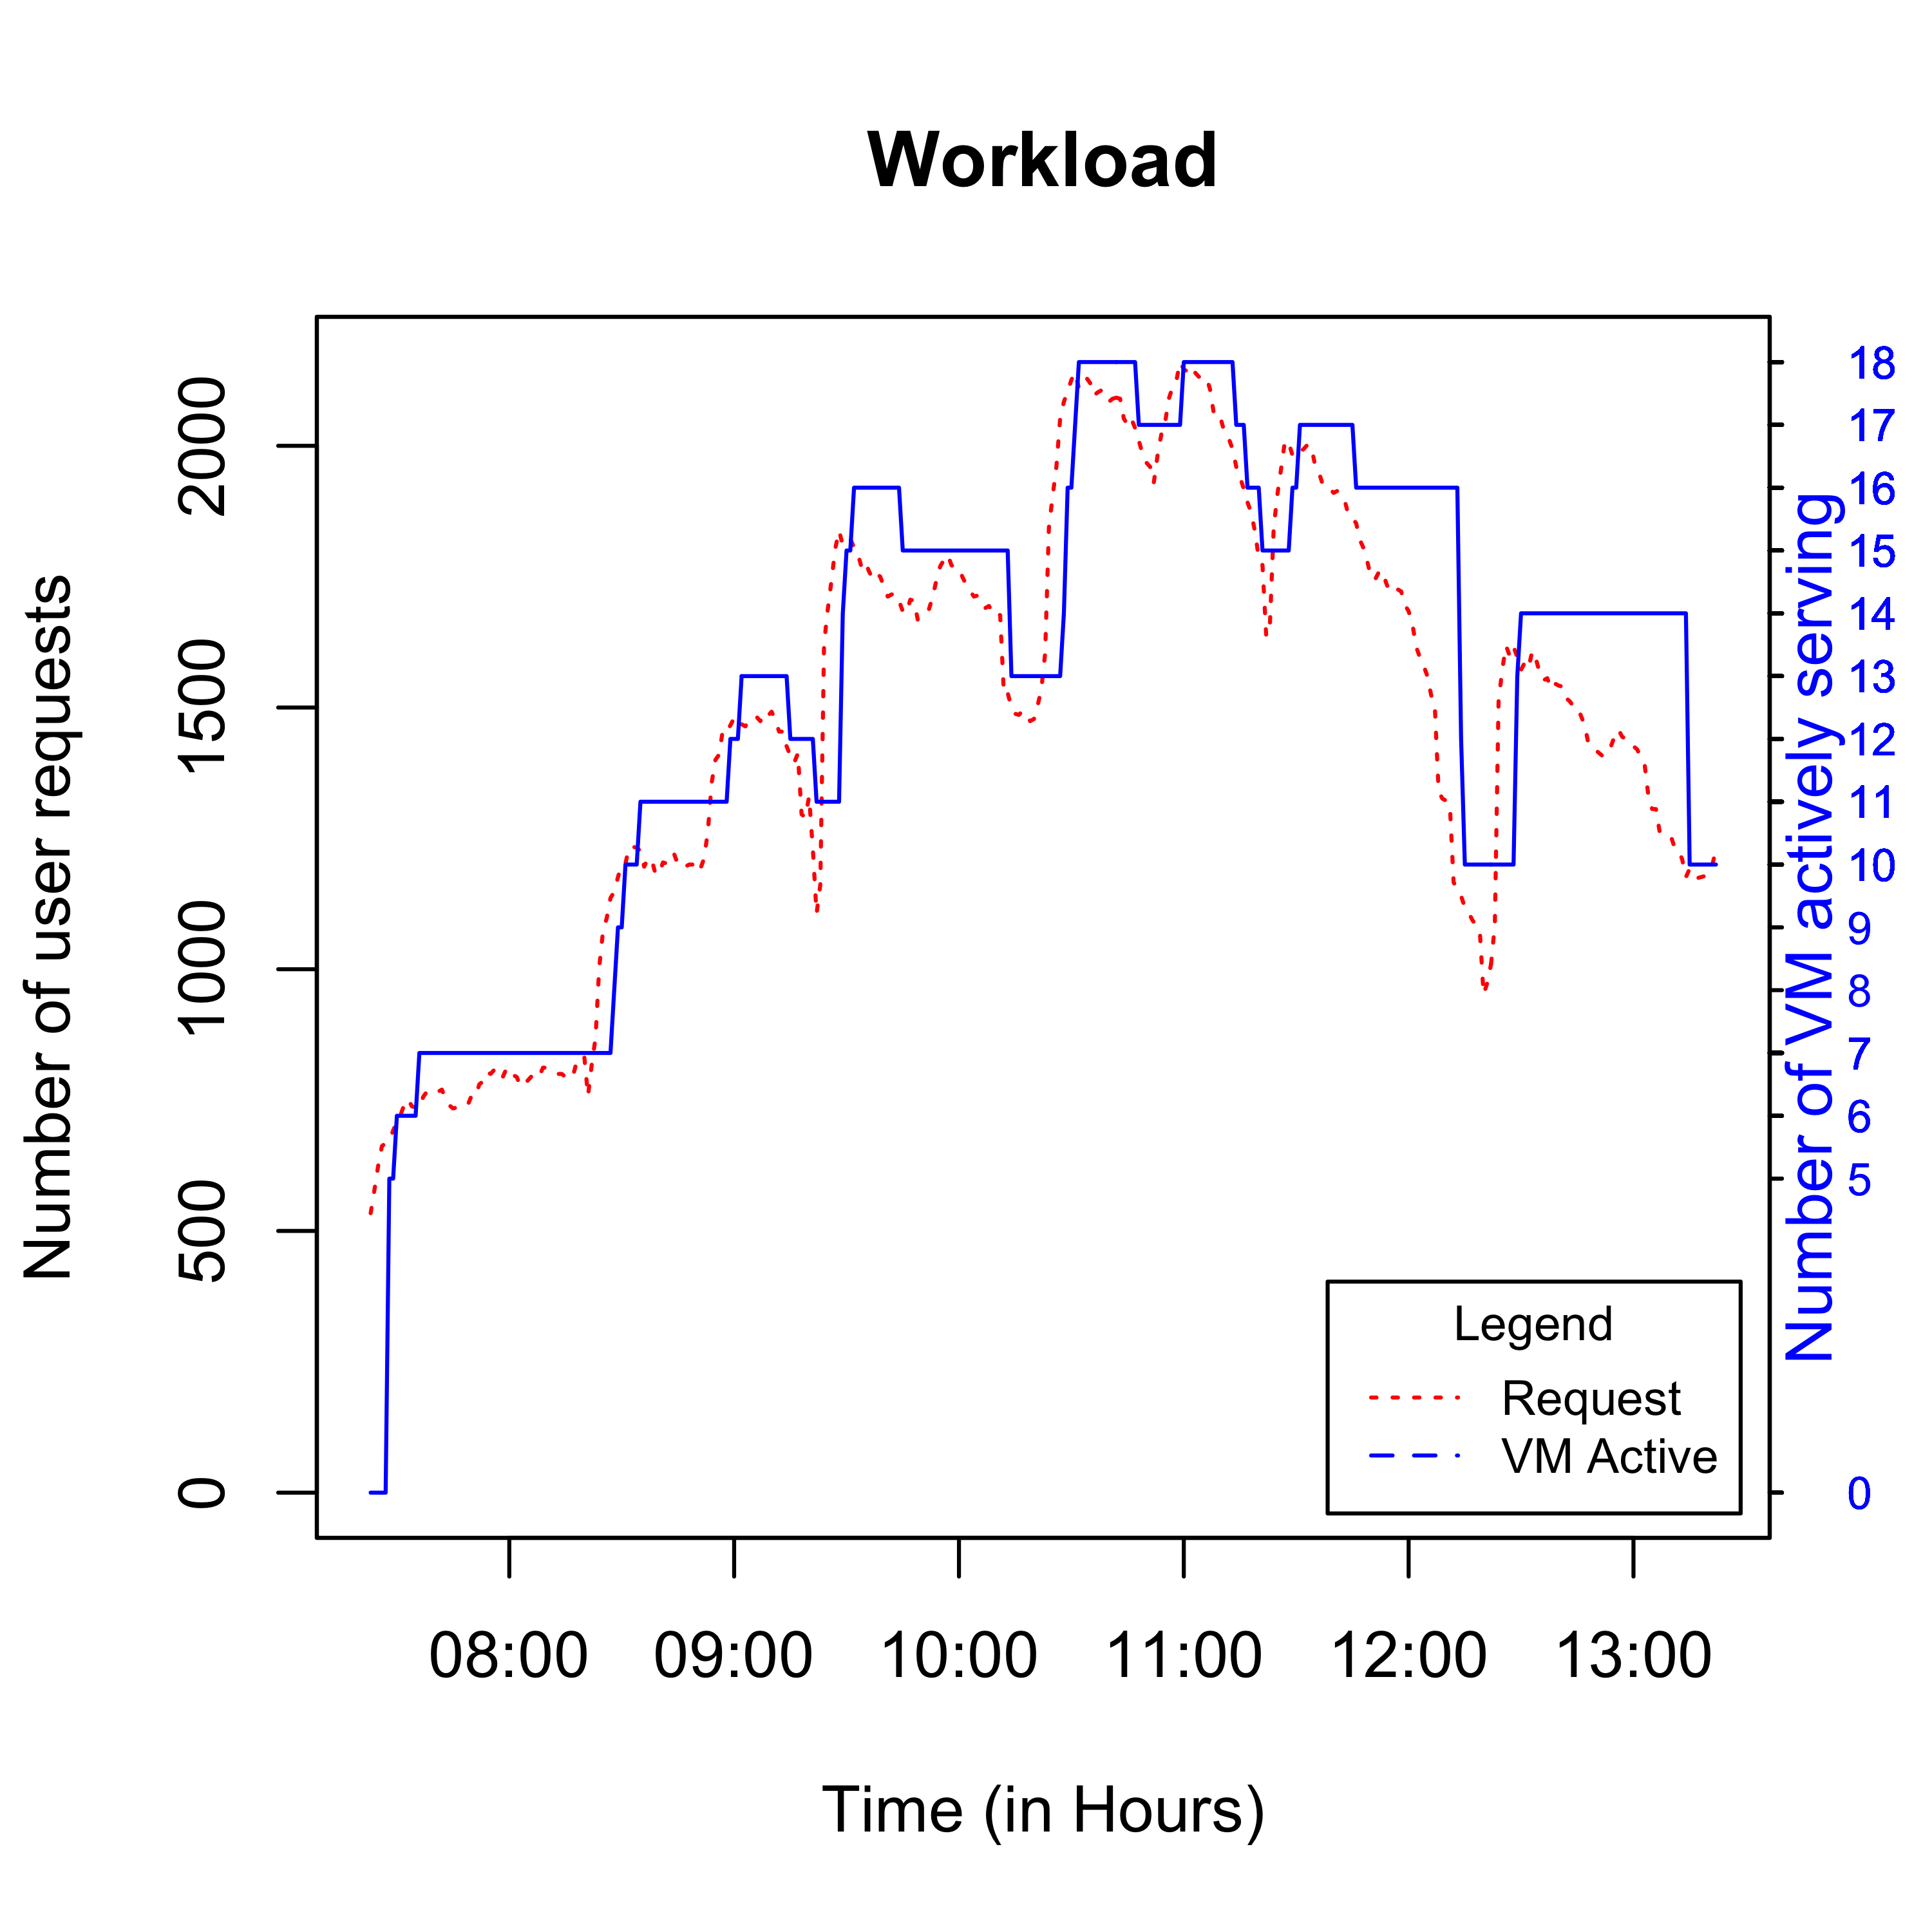
\includegraphics[width=\textwidth]{slaviolationlast.png}
         \caption{SLA Violation exmaple-2}
         \label{figure:slaviob}
     \end{subfigure}
     \caption{SLA violations}
     \label{fig:slaviolationfig}
  \end{figure}


 \section{Simulation design}
 \label{sec:Simulation design}

 \subsection{Design overview}
 \label{sub:Design overview}
 The goal of the simulation is to correctly simulate the behavior of the scaling algorithm in cloud environment from the cloud users perspective. From the cloud users perspective the cloud cost, time to resource allocation, and the VM's utilized are the most important criteria to evaluate cloud service for their cloud hosted application\cite{kim2015pics}.

 \subsubsection{Key challenges to design ElasticSim}
 \label{subs:Key challenges to design ElasticSim}
 Key challenges faced while designing ElasticSim simulator are:

 \begin{enumerate}
   \item How to model the VM without relaying on any virtualization technologies?
   \item How to handle the user requests data to provide input to the simulator?
   \item How to integrate scaling algorithm within the simulator?
 \end{enumerate}

 To solve the first challenge, ElasticSim simulator is designed to model each VM as an object. Simulator user can define diverse VM configurations and its associated cost in a configuration file. For second challenge, ElasticSim provides a data cleaning interface to clean raw data containing user requests to make it efficiently processed by the simulator. Last, to include scaling algorithm the simulator is designed such that the scaling algorithm can be easily interchanged.

 \subsubsection{Simulation Internals}
 \label{subs:Simulation Internals}
 ElasticSim is composed of three layers: Simulation configuration, Prediction and Simulation Core. Figure~\ref{figure:elasticsim} shows all the components of ElasticSim. The simulation configuration layer is responsible for accepting simulation user configurations. The workload prediction layer is responsible for generate prediction based on the specified workloads. The simulation core layer is responsible for including scaling algorithm and also responsible for providing simulation reports. Following is the detailed description about all these layers:
 \begin{itemize}
 \item Configuration Layer: Configuration layer include configuration files to configure various parameter to the algorithm such VM startup time and shutdown, instance cost, billing hour, workloads, number of user per instances as threshold, and  log files. This configuration is designed to simulate various startup/shutdown times, thresholds, workloads and cost. The workload configuration contains detailed configuration of actual and predicted workloads.
 \item Prediction Layer: The simulation prediction layer is responsible for generating the prediction based on ARIMA model and provides two output files, one for scaleup prediction workload and other are scale down prediction.
 \item Simulation Core: Simulation core is responsible for processing the workload events and invoke the scaling algorithm.
 Different components of Simulation core is as show in Figure~\ref{figure:elasticsim}. The Log parser and converter component handles workloads and cleaning the raw data so that its efficient for event processor. Simulation event processor will read each event in workload and invoke scaling algorithm. Scaling algorithm will see the workload and create/release VM instances object represented by VM component. After the scaling algorithm finishes, simulation event processor will invoke the report generator to record the logs and generate the graphs.
 \end{itemize}

 \RestyleAlgo{boxruled}
 \LinesNumbered
 \begin{algorithm}[ht]
  \KwIn{\( U_{i} \),\( B_{p} \),\( T_{start} \),\( T_{shutdown} \), \( Lookahead_{scaleup} \), \( Lookahead_{scaledown}\)}
  \KwOut{$VM_{usage}^{i}$,$VM_{cost}^{i}$}
  \While{until application is active}{
   \tcc{Get perdicted user request \( r_{i} \) in the time interval \(Lookahead_{scaleup} \)}
   \(r_{i}\) = \(max\)(getPredictedUserRequest(\(Lookahead_{scaleup}\)))\;
   \tcc{new machines \( n_{i} \) required in the interval \(Lookahead_{scaleup}\)}
   \( n_{i} = r_{i} / U_{i} \)\;
   \tcc{machines already running \( m_{i} \) at time \( t_{i} \)}
   \( m_{i} = getRunningVmInstanceCount() \)\;
   \uIf{\( n_{i} > m_{i} \)}{
     \tcc{Add more machines}
     \(newMachinesToStart =  n_{i} - m_{i}\)\;
     \lFor{ i=1 \emph{\KwTo} newMachinesToStart }{
     \tcc{New VM takes \( T_{start}\) mins to start}
     start new VM instance
     }
    }
    \uElseIf{\( n_{i} < m_{i} \)}{
    \tcc{Get predicted user request \( r_{i} \) in the time interval \(Lookahead_{scaledown}\) to check if machines can be extended billing period}
    \(r_{i}\) = \(max\)(getPredictedUserRequest(\(Lookahead_{scaledown}\)))\;
    \( n_{i} = r_{i} / U_{i} \)\;
    \(machinesToShutdown =  m_{i} - n_{i}\)\;
     \tcc{Stop machine before billing period to avoid billing to next hour since machines take \( T_{shutdown}\) mins to shutdown. Only stop machines which are nearing billing period.}
     \lFor{ i=1 \emph{\KwTo} machinesToShutdown }{ Stop VM instance ending billing period }
   }
  }
  \caption{AppElastic Algorithm with look-ahead}
  \label{algo:appelasticwithlookahead}
 \end{algorithm}

  \RestyleAlgo{boxruled}
  \LinesNumbered
  \begin{algorithm}[ht]
   \KwIn{\( U_{i} \),\( B_{p} \),\( T_{start} \),\( T_{shutdown} \), \( Lookahead_{scaleup} \), \( Lookahead_{scaledown}\), \( Cost_{ri}\), \(Cost_{odi}\), \(Count_{ri}\)}
   \KwOut{$VM_{usage}^{i}$,$VM_{cost}^{i}$,$Total_{cost}^{ri}$,$Total_{cost}^{odi}$}
   \While{until application is active}{
    \tcc{Get perdicted user request \( r_{i} \) in the time interval \(Lookahead_{scaleup} \)}
    \(r_{i}\) = \(max\)(getPredictedUserRequest(\(Lookahead_{scaleup}\)))\;
    \tcc{new machines \( n_{i} \) required in the interval \(Lookahead_{scaleup}\)}
    \( n_{i} = (r_{i} / U_{i}) - Count_{ri} \)\;
    \tcc{machines already running \( m_{i} \) at time \( t_{i} \)}
    \( m_{i} = getRunningVmInstanceCount() \)\;
    \uIf{\( n_{i} > m_{i} \)}{
      \tcc{Add more machines}
      \(newMachinesToStart =  n_{i} - m_{i}\)\;
      \lFor{ i=1 \emph{\KwTo} newMachinesToStart }{
      \tcc{New VM takes \( T_{start}\) mins to start}
      start new VM instance
      }
     }
     \uElseIf{\( n_{i} < m_{i} \)}{
     \tcc{Get predicted user request \( r_{i} \) in the time interval \(Lookahead_{scaledown}\).}
     \(r_{i}\) = \(max\)(getPredictedUserRequest(\(Lookahead_{scaledown}\)))\;
     \( n_{i} =  (r_{i} / U_{i}) - Count_{ri} \)\;
     \(machinesToShutdown =  m_{i} - n_{i}\)\;
      \tcc{Stop machine before billing period to avoid billing to next hour since machines take \( T_{shutdown}\) mins to shutdown.}
      \lFor{ i=1 \emph{\KwTo} machinesToShutdown }{ Stop VM instance ending billing period }
    }
    \(totalReservedInstanceCost = Cost_{ri} * Count_{ri} * \) Total hours of usage of each reserved instances \;
    \(totalOndemandInstanceCost = Cost_{odi} * \) Total On-demand instance used * Total hours of each On-demand instances used \;
   }
   \caption{AppElastic Algorithm}
   \label{algo:appelastic}
  \end{algorithm}

  \begin{figure}[h]
    \begin{center}
      \includegraphics[scale=0.6]{ElasticSim.png}
      \caption{ElasticSim System Design}
      \label{figure:elasticsim}
    \end{center}
  \end{figure}


 \section{Summary}
 \label{sec:Summary}
  Section~\ref{sec:AppElastic Algorithm} introduced and explain AppElastic algorithm. At first AppElastic was discussed without the capability of workload forecasting. Then the drawbacks of this approach was solved after introducing ARIMA time series forecast model. AppElastic algorithm was extended with lookahead feature so that it can provision the VM's before hand.

 In Section~\ref{sec:Simulation design} to test the algorithm in a simulation environment ElasticSim simulator design was introduced. Here  the concepts and ideas of simulator was introduced and explained. It also introduced how ElasticSim helps modeling cloud environment without having to interact with cloud service provider or virtualization technologies.
